\documentclass[12pt]{ecsproject}     % Use the Project Style

\graphicspath{{./figures/}}

\usepackage{lscape}
\usepackage{natbib}            % Use Natbib style for the refs.
\usepackage{listings}
\usepackage[nottoc]{tocbibind} %this will add bibliography to toc
\hypersetup{colorlinks=false}   % Set to false for black/white printing
%% ----------------------------------------------------------------
%% Definitions.tex
%% ---------------------------------------------------------------- 
\newcommand{\BibTeX}{{\rm B\kern-.05em{\sc i\kern-.025em b}\kern-.08em T\kern-.1667em\lower.7ex\hbox{E}\kern-.125emX}}

%% People
\newcounter{address}
\setcounter{address}{1}
\renewcommand{\theaddress}{\textsuperscript{\fnsymbol{address}}}
\newcommand{\address}[1]{\refstepcounter{address}\theaddress#1\\}
\newcommand{\Name}[3]{\texorpdfstring{\href{mailto:#3}{#2}#1}{#2}\xspace}
\newcommand{\SteveRGunn}[1]{\Name{#1}{Steve R. Gunn}{S.R.Gunn@ecs.soton.ac.uk}}

%% Dingbats
\newcommand{\tick}{\ding{51}}
\newcommand{\cross}{\ding{55}}

%% Calculus
\newcommand{\pd}[2]{\ensuremath{\frac{\partial #1}{\partial #2}}\xspace}
\newcommand{\fd}[2]{\ensuremath{\frac{d #1}{d #2}}\xspace}
\newcommand{\dint}{\ensuremath{\int\!\!\!\int}\xspace}
\newcommand{\tint}{\ensuremath{\int\!\!\!\int\!\!\!\int}\xspace}

%% Math Sets
\newcommand{\Q}[1]{\ensuremath{\mathbb{#1}}\xspace}
\newcommand{\R}{\Q{R}}

%% Matrix, Vector
\newcommand{\V}[1]{\ensuremath{\boldsymbol{#1}}\xspace}
\newcommand{\M}[1]{\ensuremath{\boldsymbol{#1}}\xspace}
\newcommand{\0}{\V{0}}
\newcommand{\1}{\V{1}}
\newcommand{\I}{\M{I}}

%% Math Functions
\newcommand{\F}[1]{\ensuremath{\mathrm{#1}}\xspace}
\newcommand{\sgn}{\F{sgn}}
\newcommand{\tr}{\F{trace}}
\newcommand{\diag}{\F{diag}}

%% Math Names
\newcommand{\N}[1]{\ensuremath{\mathit{#1}}\xspace}

%% Data
\newcommand{\mc}[1]{\ensuremath{\mathcal{#1}}\xspace}
\newcommand{\Hyp}{\mc{H}}
\newcommand{\D}{\mc{D}}

%% Kernel
\newcommand{\K}{\M{K}}
\newcommand{\eins}{\texorpdfstring{\ensuremath{\epsilon}}{\textepsilon}-insensitive\xspace}
\newcommand{\e}{\ensuremath{\epsilon}\xspace}
\newcommand{\Bxi}{\ensuremath{\boldsymbol{\xi}}\xspace}
\newcommand{\Kanova}{\ensuremath{\mathit{K_{ANOVA}}}\xspace}
\newcommand{\Kspline}{\ensuremath{\mathit{K_{spline}}}\xspace}

%% Bayesian
\newcommand{\MP}{\ensuremath{\mathit{{\scriptscriptstyle \hspace{-1.5pt}M\hspace{-1.5pt}P}}}\xspace}
\newcommand{\ML}{\ensuremath{\mathit{{\scriptscriptstyle \hspace{-1.5pt}M\hspace{-1.5pt}L}}}\xspace}
\newcommand{\Qw}{\ensuremath{Q_{\w}(\w)}\xspace}
\newcommand{\Qa}{\ensuremath{Q_{\Ba}(\Ba)}\xspace}
\newcommand{\Qb}{\ensuremath{Q_{\beta}(\beta)}\xspace}
\newcommand{\wMPab}{\ensuremath{\w_{\MP|\bar {\Ba},\bar \beta}}\xspace}
\newcommand{\wMP}{\ensuremath{\w_{\MP}}\xspace}
\newcommand{\yMP}{\ensuremath{y_{\MP}}\xspace}
\newcommand{\BaMP}{\ensuremath{\Ba_{\hspace{1pt}\MP}}\xspace}
\newcommand{\aMP}{\ensuremath{\alpha_{\hspace{1pt}\MP}}\xspace}
\newcommand{\bMP}{\ensuremath{\beta_{\hspace{1pt}\MP}}\xspace}
\newcommand{\Sab}{\ensuremath{\M{\Sigma}_{\bar \Ba,\bar \beta}}\xspace}
\newcommand{\Ba}{\ensuremath{\boldsymbol{\alpha}}\xspace}
\newcommand{\Bb}{\ensuremath{\boldsymbol{\beta}}\xspace}
\newcommand{\Bm}{\ensuremath{\boldsymbol{\mu}}\xspace}
\newcommand{\BL}{\ensuremath{\boldsymbol{\Lambda}}\xspace}
\newcommand{\BPhi}{\ensuremath{\boldsymbol{\Phi}}\xspace}
\newcommand{\SMP}{\ensuremath{\M{\Sigma}_{\MP}}\xspace}

\newcommand{\Pa}{\ensuremath{P(\alpha|\mathcal{H})}\xspace}
\newcommand{\Pb}{\ensuremath{P(\beta|\mathcal{H})}\xspace}
\newcommand{\Pab}{\ensuremath{P(\alpha,\beta|\mathcal{H})}\xspace}
\newcommand{\Pw}{\ensuremath{P(\w|\mathcal{H})}\xspace}
\newcommand{\PD}{\ensuremath{P(\D|\mathcal{H})}\xspace}
\newcommand{\PwIa}{\ensuremath{P(\w|\alpha,\mathcal{H})}\xspace}
\newcommand{\PDIwb}{\ensuremath{P(\D|\w,\beta,\mathcal{H})}\xspace}
\newcommand{\PDwab}{\ensuremath{P(\D,\w,\alpha,\beta|\mathcal{H})}\xspace}
\newcommand{\PDIw}{\ensuremath{P(\D|\w,\mathcal{H})}\xspace}
\newcommand{\PwID}{\ensuremath{P(\w|\D,\mathcal{H})}\xspace}
\newcommand{\PwabID}{\ensuremath{P(\w,\alpha,\beta|\D,\mathcal{H})}\xspace}

\newcommand{\PanH}{\ensuremath{P(\alpha)}\xspace}
\newcommand{\PbnH}{\ensuremath{P(\beta)}\xspace}
\newcommand{\PabnH}{\ensuremath{P(\alpha,\beta)}\xspace}
\newcommand{\PwnH}{\ensuremath{P(\w)}\xspace}
\newcommand{\PDnH}{\ensuremath{P(\D)}\xspace}
\newcommand{\PwIanH}{\ensuremath{P(\w|\alpha)}\xspace}
\newcommand{\PDIwbnH}{\ensuremath{P(\D|\w,\beta)}\xspace}
\newcommand{\PDwabnH}{\ensuremath{P(\D,\w,\Ba,\beta)}\xspace}
\newcommand{\PDIwnH}{\ensuremath{P(\D|\w)}\xspace}
\newcommand{\PwIDnH}{\ensuremath{P(\w|\D)}\xspace}
\newcommand{\PwabIDnH}{\ensuremath{P(\w,\alpha,\beta|\D)}\xspace}

\newcommand{\PDwBab}{\ensuremath{P(\D,\w,\Ba,\beta|\mathcal{H})}\xspace}
\newcommand{\PwIBa}{\ensuremath{P(\w|\Ba,\mathcal{H})}\xspace}
\newcommand{\PBab}{\ensuremath{P(\Ba,\beta|\mathcal{H})}\xspace}
\newcommand{\PwBabID}{\ensuremath{P(\w,\Ba,\beta|\D,\mathcal{H})}\xspace}

\newcommand{\PBanH}{\ensuremath{P(\Ba)}\xspace}
\newcommand{\PwIBanH}{\ensuremath{P(\w|\Ba)}\xspace}

%% Snakes
\newcommand{\Esnake}{\ensuremath{\mathit{E_{snake}}}\xspace}
\newcommand{\Eimage}{\ensuremath{\mathit{E_{image}}}\xspace}
\newcommand{\Econt}{\ensuremath{\mathit{E_{cont}}}\xspace}
\newcommand{\Ecurv}{\ensuremath{\mathit{E_{curv}}}\xspace}
\newcommand{\Eint}{\ensuremath{\mathit{E_{int}}}\xspace}
\newcommand{\Eext}{\ensuremath{\mathit{E_{ext}}}\xspace}
\newcommand{\Eterm}{\ensuremath{\mathit{E_{term}}}\xspace}
\newcommand{\Eline}{\ensuremath{\mathit{E_{line}}}\xspace}
\newcommand{\Eedge}{\ensuremath{\mathit{E_{edge}}}\xspace}
\newcommand{\Econ}{\ensuremath{\mathit{E_{con}}}\xspace}
\newcommand{\Eangle}{\ensuremath{\mathit{E_{angle}}}\xspace}
\newcommand{\Elshape}{\ensuremath{\mathit{E_{lshape}}}\xspace}
\newcommand{\Eedgedir}{\ensuremath{\mathit{E_{edgedir}}}\xspace}
\newcommand{\Emodel}{\ensuremath{\mathit{E_{model}}}\xspace}
\newcommand{\wte}{\ensuremath{\mathit{w_{term}}}\xspace}
\newcommand{\wli}{\ensuremath{\mathit{w_{line}}}\xspace}
\newcommand{\wed}{\ensuremath{\mathit{w_{edge}}}\xspace}
\newcommand{\wco}{\ensuremath{\mathit{w_{con}}}\xspace}

%% Environments
\newcounter{alg}
\newenvironment{algorithm}[1]
{
    \stepcounter{alg}
    \begin{table}[htb]
    \centering
    \begin{tabular}[t]{ll}
    \hline&\\
    \multicolumn{2}{l}{\bf Algorithm \arabic{alg}: #1}\\&\\
} {
    &\\
    \hline
    \end{tabular}
    \end{table}
}
            % Include your abbreviations

%
%
%
%
%

\begin{document}
\frontmatter
\addresses{\goupname \\ \deptname \\ \univname}
\authors{\texorpdfstring
		{\href{mailto:dpm3g10@ecs.soton.ac.uk}{ Dionisio Perez-Mavrogenis}}
		{Dionisio Perez-Mavrogenis}
		}
\date{\today}
\title{Andron: a site maintenance framework.}

\supervisor{Dr. Rogers,A.}
\examiner{Dr.Thomas, K.S.}

\degree{MEng Computer Science with Artificial Intelligence}

\maketitle
\section*{\textit{Abstract}}
This report will describe what the \emph{Andron} project is all about, the technologies used in building the framework and give a summary of what has been accomplished so far and what else is to be implemented in order to complete the \emph{Andron} project. \\

In short, \emph{Andron} is a framework for reporting maintenance and other issues which cause the disrupt of services in any given site that has registered with the \emph{Andron} service. That is made possible using a combination a mobile application that runs on smartphones and a web application that resides on a server. \\

The idea behind \emph{Andron} is to allow for a smaller response time in fixing reported issues that might disrupt or completely prohibit the use of the facilities or services of a site by the clients, and it is also meant to increase awareness regarding a problem by allowing users of the service to see what others have reported. Furthermore, \emph{Andron} is meant to be usable both by large or small organizations of any kind.\\

\emph{Andron} was inspired by the poor response of the government towards filed reports from citizens regarding breakage of public property in my country, Greece.

\tableofcontents
\mainmatter

\section{Acknowledgements and Statement of Originality}

This project would not be in its current state if several people had not contributed both their time and their knowledge.

First and foremost my supervisor, Dr. Alex Rogers, who helped me get a solid project definition and has been providing ideas (like the use of the Phonegap framework), as well as material support (by providing me with an actual phone to test the code on) and pointing me towards sources of information and has been willing to help with anything.

Another person I would like to extend my gratitude towards is James McInerney , a researcher for the ECS. Dr. Rogers put us in contact, as Mr. Mcinerney has developed a Phonegap application with similar capabilities, and so could provide more technical advice. James has been really willing to help since our first meeting, and has been prompt to reply on questions.

Last but not least, I would like to thank my second examiner, Dr. Ken Thomas, for pointing out useful suggestions and ideas for the project, and Mr. Garry Niblett , senior business change manager for the Estates and Facilities department, for his support for the initial Planon proposal.


\paragraph{Originality} The code I am writing is my own, and any external source code will be clearly referenced. Any help or troubleshooting will also be credited where it is due.

\newpage
\section{Introduction}

There exist multiple tools in the market for performing assets maintenance management, but there is no simple and inexpensive solution for small organisations to manage maintenance of their assets. Furthermore, the existing tools do not allow the facilities' users to contribute in reporting maintenance faults, speeding up the repair process. 

This is what Andron attempts to solve, to provide small organisations with an easy, inexpensive, accessible framework for performing maintenance management and allowing their users to participate in that process, minimising the time from the identification of an issue till the time it gets fixed.

Andron is, principally, a framework that will allow easier and more efficient site and facilities maintenance. It does so by using an application that will run on smart-phones and an application that will be running on a web-server\footnote{Andron website : (\hyperlink{http://andron.zymichost.com}{http://andron.zymichost.com})}.

The owners of a site or facilities will register with the Andron application and become \textbf{Andron Authorities}. Users will be able to download and install a copy of the Andron application on their smart-phones, point the application to the Andron authority that they want to file a maintenance report with. The main motivation behind Andron is to allow users of a facility or site to contribute to the maintenance of the respective facilities by filing reports about maintenance issues as they spot them on the go, and not have to go and sit on a desktop computer and file that through a website (because most users will probably forget about that). This way issues that require attention will be dealt with faster and be less disruptive to other users.

With each of their reports, the users will be able to attach a photograph of the problem, while at the same time their geographical location will be determined by the phone's GPS system (if any), and a geo-tagged photograph will be uploaded to the Andron server, along with a title and a description for the issue being reported. 

Users will be able to see the resolution status of the reports they have filed for a given Andron Authority and of other reports they might have saved as their favourites, get a list of the most recently filed reports, visualize those on a map and get information on the resolution status of each report. That way, users share information with each other as well rather than just making the job of the maintenance team easier. Each request will be tied to a particular MAC address, and users will have the option to provide their details (first and last name and a contact email address) with each submission, or post anonymously.

The administrator's version of the smart-phone application application will have a similar user interface to the user version, but will feature some additional administrative functionality. Administrators will have the option to perform filtered queries over all filed reports, view a users history (and also disallow them from submitting more reports, as a result of false or inaccurate reports the users have filed), toggle the resolution status of a report, remove a filed report.

The purpose of the web application will be two-fold. 

The website will have a landing page where owners willing to implement Andron will register and become Andron Authorities, and a section where Andron Authorities will be able to login to manage their sites, and perform many of the actions that are located on the administrator's version of the Andron smart-phone application.

The second purpose of the Andron website will be to interact with the smart-phone applications, either by providing content to them (for example the latest reports for a given Andron Authority) or by performing actions sent by the application users (favouring a report, submitting a new report or toggling the status of a report, just to name a few). Also, the web-application will also manage the databases on the server ( a separate database for each Andron Authority and a database central to the application for storing the details of various Andron Authorities).

There is one similar application to Andron that exists already in the market. It is called the Boston Citizens Connect\footnote{Application website :\hyperlink{http://www.cityofboston.gov/DoIT/apps/citizensconnect.asp}{http://www.cityofboston.gov/DoIT/apps/citizensconnect.asp}}, and it is has been used as a reference for drafting the requirements.

\pagebreak
\section{High Level Technical Overview}
In this section, a high level overview of the architecture that will be used in the Androd project is outlined.

\subsection{Tools and techniques used}
For developing mobile phone applications, vendors usually provide their own virtual devices for testing. 

Testing on a virtual platform rather than on an actual phone has several benefits, like eliminating the danger of potentially crashing the phone or losing data, it is easier to test for different versions of the operating system and doesn't require an actual device, amongst others.

However, testing on a virtual platform has got several drawbacks as well. Unique device features like the camera or the GPS can not be used (although the Android Virtual Devices are able to emulate use of the camera), and so one never really knows if the code will work in production. Also, testing on a computer doesn't give an actual estimate of the display quality of the application on the devices or the performance, given that the emulator runs on the computer and so has generally got more resources available when running.For this reason, my supervisor supplied me with an Android phone to test my code on. 

To avoid crashing the phone, the code if first compiled and run on an Android virtual device, and when it is necessary to use functions which are not available to the emulator (like the GPS, for example) then I upload the application to the phone.

For development purposes, the Eclipse development environment is used with the Google Android development plug-in, which provides access to the ADB(Android Debug Bridge, the official debugger), the Android Emulator and the various versions of the Android SDK.

Building of the application is done through Phonegap Build \footnote{Phonegap Build Service website : \hyperlink{http://build.phonegap.com/}{http://build.phonegap.com/}} and after is has been build, it is downloaded from the Phonegap Build website and installed on the phone.


\subsection{Smart-phone application technical specifications}
Originally, Andron was to be implemented in Java, as a native Android application. After Dr.Thomas pointed out that this would ignore a massive amount of users that use other smart-phones (like iPhones or Blackberry phones), Dr.Rogers suggested that the project implementation be changed, and finally Andron was decided to be implemented with the Phonegap\footnote{Phonegap website :  \hyperlink{http://phonegap.com/}{http://phonegap.com/}} framework.

 In short, the Phonegap framework allows the development of cross-platform applications in Javascript, CSS and HTML, and provides Javascript APIs for accessing native operating system functions and for accessing the hardware(like the ability to use the camera, for example). The Phonegap Build Service then takes the developed code and packages it according to the specified format that each operating system requires that their applications be packaged.

There are several factors that need to be taken into account while designing software for mobile devices. Programmers need to be aware of the computational limitations of mobile devices (limited amount of CPU power, amounts of RAM and phone memory storage) and battery lifetime, amongst others, as well as a limited display size. Another issue that developers need to take into account is that different devices, with different hardware specifications, running different versions of the same operating system will have to support as much of the features of the application as possible, and thus implementing version-specific features should mostly be avoided.

As of this writing, the proposed technologies used to develop the application are summarized in the following list, which is not exhaustive or final, as these technologies might change if circumstances require such an action :
\begin{itemize}
	\item Javascript
	\item HTML5 \footnote{W3C HTML5 specification : \hyperlink{http://www.w3.org/TR/html5/}{http://www.w3.org/TR/html5/}} 
	\item CSS3 \footnote{W3C CSS3 specification : \hyperlink{http://www.w3.org/TR/CSS/\#css3}{http://www.w3.org/TR/CSS/\#css3}} 
	\item jQuery \footnote{jQuery website : \hyperlink{http://jquery.com/}{http://jquery.com/}}
	\item jQueryMobile \footnote{ jQueryMobile website :  \hyperlink{http://jquerymobile.com/}{http://jquerymobile.com/}} 
	\item Google Maps Javascript API V3 \footnote{ Maps API V3:  \hyperlink{https://developers.google.com/maps/documentation/javascript/}{https://developers.google.com/maps/documentation/javascript/}} 
\end{itemize}

jQuery is a Javascript library that aims to reduce development time and effort by abstracting away browser-specific Javascript quirks, resulting in much more readable code.

jQueryMobile is an HTML5 user interface system optimized for displaying data to mobile devices and tablets. jQueryMobile will be used to easily style the user interface of Andron, provide better graphics and a more familiar "look-and-feel" for the application, and for making the application's look consistent across different operating systems.

The Google Maps API will be used for allowing the users to visualise all the reports on the map, and for positioning themselves on the map more accurately. The GPS coordinates will be used to retrieve the map tile from Google, and then the users will further refine their position on the map. This way, each report will have a more precise location associated with it, rather than a general one, as GPS is not always very accurate.

\subsection{Web application technical specifications}
The web application will be somewhat more straightforward to implement, because it will involve the typical development of a website, both the front-end and the back-end. The development of this website is no different than the development of any other website and should conform the web design standards defined by the World Wide Wed Consortium \footnote{W3C web design standards : \hyperlink{http://www.w3.org/standards/webdesign/}{http://www.w3.org/standards/webdesign/}}

The fronted will be powered by Javascript (and associated libraries like jQuery), HTML5 and CSS3. 

The server-side scripting of the back-end will be done in the PHP programming language, and the database engine that will be used is MySQL. The combination of PHP and MySQL to power dynamic content-driven websites has been proven through the multiple websites that are powered by this combination and I also have personal experience developing such applications. There are a lot of resources on-line for troubleshooting issues and guides for implementing functionality, and both PHP and MySQL have got really big communities supporting them.

The web application will not only be used to power the Andron Authority registration process, but also to deliver content to the applications, file reports sent to the server, manage the database of each Andron Authority and more.

\pagebreak
\section{Documentation Accompanying Andron}

As this is somewhat of a large project to be completed by one person alone appropriate documentation has to exist in order to have a well-defined goal, the technologies and techniques that are to be used to implement the project and a time frame for completion of the application.

The two most essential documents that attempt to define the application are the "Requirements Document", which define exactly what features an application will have, and the wireframes, which tell the designers how the application will look like. Some use cases have been devised as well, in order to check that the final products meets all of the requirements.

An initial draft of both of these documents were produced in the beginnings of the project, even before prototyping began. The Requirements Document is included in Appendix A.1 and the Use-Cases are included in Appendix A.2.

The technologies that should be used to bring this project to completion are also described in the requirements document, and are more explicitly defined in Section 0.3 .

Last but not least, the time schedule for completing the application is being maintained as a Gantt chart, with what has been done up until now being show in Section 0.6 and the chart for future progress being show in Section 0.7. The software chosen for creating and managing the Gantt charts was GanttProject, a cross-platform open source software.

Additionally, every working file for the Andron project is being version controlled using Git\footnote{Github website\hyperlink{http://github.com}{http://github.com}} version control system. working files for the Andron project that are being version-controlled do not only include the source code for the project, but documentation files as well, deliverables and even media files being used for the application.

\pagebreak
\section{Relevant Literature}

Mobile application development,in contrast to desktop application development, is new and as a result suffers from a lack of established software development patterns\cite{ken}. This leaves a window of opportunity open for new patterns to emerge, but also poses a risk for amateur developers due to lack of guidance and established principles, leading to the development of poor or insecure code and bad programming habits.

However, there is not a complete lack of sources of information. To promote good style, major operating system designers have guidelines on what they promote as best practices for designing applications for their systems\footnote{Android\hyperlink{http://developer.android.com/design/index.html}{http://developer.android.com/design/index.html},\\ Blackberry\hyperlink{http://docs.blackberry.com/en/developers/?userType=21}{http://docs.blackberry.com/en/developers/?userType=21},\\  iOS \hyperlink{http://developer.apple.com/library/ios/navigation/}{http://developer.apple.com/library/ios/navigation/}}, and a lot of books exist on developing applications for these operating systems.

Another problem that we are faced with because of using the Phonegap framework for developing Andron is that the framework is somewhat new and not a lot of literature exists on how to use it. However, there are still some resources available on-line which I consider to be of high quality. More specifically, websites like StackOverflow\footnote{\hyperlink{http://stackoverflow.com/}{http://stackoverflow.com/}}, the GoogleGroups threads discussing Phonegap and the official Phonegap API guides provide very valuable resources for getting started, and a lot of assistance with troubleshooting or recommending alternative approaches for developing applications. Additionally, \emph{Phonegap Mobile Application Development Cookbook}\cite{pgcook} by Matt Gifford is a book extending the basic Phonegap API guides with more advanced features, and the Phonegap Blog\footnote{Phonegap Blog\hyperlink{http://phonegap.com/blog}{http://phonegap.com/blog}} provides articles on how to manage a project and recommended practices when using Phonegap.

\pagebreak
\section{Progress so far}

Progress so far is steady, although it might not seem a lot. As of this report, the server for the Andron application has been registered under the domain name \hyperlink{http://andron.zymichost.com}{http://andron.zymichost.com}, the wireframes have been produced and a prototype application has been produced, which demonstrates the key functionality of the final product. The prototype was tested on a virtual device, as well as the Android phone that the ECS provided me with.

Figure 1 demonstrates then Gantt chart of the work that has been completed to date, and the progress of each.

Although it appears that actual work has not being carried out until mid-November, that is not true. From October $3^{rd}$ up  until October $12^{th}$(the deadline for the project brief), I was meeting with my supervisor trying to establish my individual project topic, and the result was to create an application offering mobile support for Planon\footnote{UoS Planon service: \hyperlink{https://planon.soton.ac.uk/}{https://planon.soton.ac.uk/}} . From then onwards, up early November I was meeting with university staff responsible for the operation of the Planon service in our university, which turned out to be fruitless, in part both to the commitment required by the University of Southampton for developing software for them, as well as for the reasons mentioned in the Introduction. After that conclusion, we decided to reconsider the topic of the individual project and implement the Andron framework.

In reality, Figure 1 shows only the work that was carried out for implementing a prototype of Andron, and not all the work and meetings that led to the shift in focus that created Andron.

\begin{landscape}
\begin{figure}
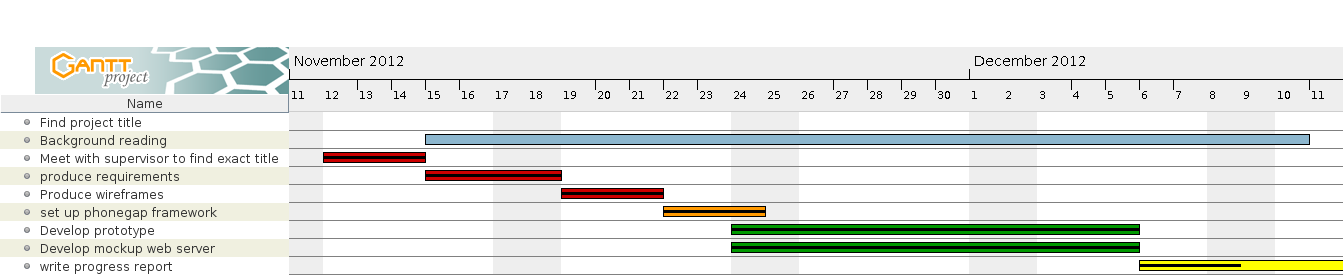
\includegraphics[scale=0.5]{proto.png}
\caption{Gantt chart for all the work that has been currently done (November $12^{th}$ - December $11^{th}$).}
\end{figure}
\end{landscape}

\pagebreak
\section{Future work}
The remaining of the work has been broken down on the five major sections that exist, with details of each section being omitted (as they are currently unknown). The five major sections of work that need to be carried out are :

\begin{enumerate}
\item Client application
\item Administrator application
\item Server application development
\item Testing
\item Writing of final report
\end{enumerate}

Figure 2 shows the Gantt chart for the remaining work.

One might observe that the development slots for the user and administrator application overlap with the development slot for the server application. That is intentional, as functionality will be added to both incrementally as the project moves forward. That will help identify and develop the exact needs of each component. The administrator's application can, and will, be developed separately from the user's application, because the functionality of one does not depend on the other, while the functionality of both depends on an existing and operational server.

There has been a lot of time left for testing, but that is done on purpose. While testing simply entails verifying the security of the application, it is sometimes really hard and time consuming to figure out where things go wrong. Another reason for giving testing so much time is to account for any delay that might occur in the development phase (by other academic obligations or otherwise).

Although this Gantt chart is a good starting point, it should not be considered final for the aforementioned reasons.

\begin{landscape}
\begin{figure}
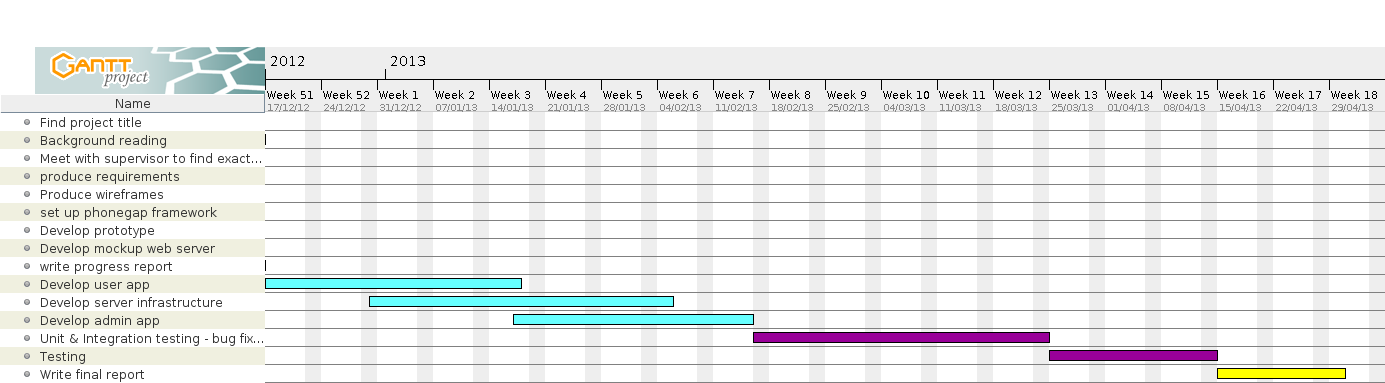
\includegraphics[scale=0.5]{rem.png}
\caption{Overview of the major blocks of work that are to be completed for the project.}
\end{figure}
\end{landscape}

\pagebreak
\section{Conclusion}
In conclusion, this application ,although straightforward as a concept, requires a lot of involvement and reading around the subject if the application is to be considered quality software. The project has got aspects that are heterogeneous in nature (mobile application and server application development), which require different approaches, resulting in an increased workload.

Progress so far is satisfactory and every deadline has been met. However, other coursework obligations might prolong the development time for certain aspects of the application, something that will have be taken into account when planning the remainder of the work, without that having a negative impact on the quality of the application.

%
%
%
%
%
%
%
%
%
%

\appendix
\chapter{Documentation}
\section{The Requirements Document}
\textbf{Terminology:}
Andron Authority : A business/person that has deployed the Andron system to their facilities

\textbf{Target Operating System }: Cross platform application developed with the Phonegap framework.

\textbf{Mobile application Requirements :}

\textbf{Proposal :} Have a client application and a admin application with similar functionality, but allow administrators more actions. 

\textbf{Functional Requirements for client application:}
\begin{enumerate}
\item Read Andron Authority information through QR codes or manual insertion
\item Provide problem description
\item Provide problem details
\item Provide ability to attach picture with the report
\item Provide ability to locate position of report
\item Identify each user uniquely
\item  Ability for anonymous posting 
\item  Provide ability to insert full name
\item  Provide ability to insert email 
\item  Have a list of the most recent reports
\item  Allow a user to add and remove a report from favourites
\item  Visualise reports on a map
\item  Allow users to up-vote a report
\end{enumerate}

\textbf{Functional Requirements for admin app :}
\begin{enumerate}
\item  Administrator MUST login to authenticate himself as an administrator.
\item  View a report
\item  Toggle the status of a report
\item  Display reports on a map
\item Browse recent reports
\item Delete a report
\item Ban a user
\item Change password
\end{enumerate}

\textbf{Optional Non-Functional Requirements for both applications:}
\begin{enumerate}
\item Have a clean, intuitive interface
\item No deep/obscure/hidden sub-menus
\item Provide help to application user, pointing them to information authorities
\end{enumerate}

\textbf{Web application requirements}
The web application will be written in PHP and the database backend will be MySQL.

\textbf{Administrator's Interface:}
\begin{enumerate}

\item  Add more administrators (only for the one who registered the AndronAuthority)
\item Manage administrators (only for the one who registered the AndronAuthority)
\item Toggle status of a report
\item Change account password
\item Ban a user
\item Delete a report
\item Browse reports
\item Visualise reports on a map
\item  View a report
\item Remove themselves from the service  (only for the one who registered the AndronAuthority)
\end{enumerate}
\textbf{Non-Functional Requirements for both interfaces:}
\begin{enumerate}
\item Have a clean and intuitive interface
\item Don't diverge too much from the mobile versions.
\item No deep/obscure/hidden sub-menus.
\item Provide help to application user, pointing them to information authorities
\item Make it as HTML5 and CSS3 compliant as possible
\end{enumerate}

Proposed server application architecture
The server application running on the Andron website will be responsible for managing a set of databases, one for keeping records of the application and one for each Andron Authority.

Databases for Andron Authorities will be used to store information about reports, an administrators list (containing at least usernames, passwords and their tokens for the session – the later are for security purposes) and a blacklists of users not allowed to submit reports, possibly adding more tables if necessary.

The database for the application will hold information on AndronAuthorities (such us owner name and credentials, their QR codes, their database names, administrator credentials for logging in and possibly other information).

The server application architecture or functionality shall be updated as required.

\section{Use Cases}
Use cases for checking that Andron application functional requirements have been met.

\begin{itemize}
\item 1. Facility owner wants to deploy system to their facility, process of getting it. 
\item 2. Facility owner wants to let his clients know of the system. 
\item 3. Facility owner wants to add or remove an Administrator. 
\item 4. Client wants to install the application. 
\item 5. Client wants to connect application with said facility. 
\item 6. Client wants to submit report. 
\item 7. Client wants to browse recent reports. 
\item 8. Client wants to view report info. 
\item 9. Client wants to see reports on the map. 
\item 10. Client wants to up-vote on a reported issue.
\item 11. Allow a client to refresh the list of reported issues. 
\item 12. Administrator of said Andron Authority wants to review a report and change its status. 
\item 13. Administrator of said Andron Authority wants to block a user of the application. 
\item 14. Test administrator functionality via the web-interface.
\end{itemize}

\bibliographystyle{plain}
\bibliography{bibl}

\end{document}